\chapter{实验几何}

几何学是研究“空间”的形体和性质的科学。“空间”
就是我们和万物以至星象天体共存的所在。在日常生活中,
我们举目四望所见到的地方,都是空间的一部分。同学们在
小学数学课中学过的柱体、锥体、球体等等,它们都各自占
有空间的一部分,并且构成不同的形体。各种形体的种种性
质,如各部分的长度、角度、面积,以及体积等等。都是在
我们的生活和生产实践中所不可缺少的知识。
\begin{figure}[htp]
	\centering
\begin{tikzpicture}[scale=.7]
\begin{scope}
	\draw (1.5,0) ellipse [x radius=1.5, y radius=.5];
	\shade (0,0) rectangle (3,4);
	\shade (1.5,4)[draw] ellipse [x radius=1.5, y radius=.5];
	\draw (0,0)--(0,4);
	\draw (3,0)--(3,4);
		\node at (1.5,-1.5){圆柱};

\end{scope}
\begin{scope}[xshift=5.5cm]	
	\shade (1.5,0)[draw] ellipse [x radius=1.5, y radius=.5];
		\fill[gray!50] (0,0)-- (3,0)--(1.5,4)--(0,0);
		\draw (0,0)--(1.5,4)-- (3,0);
	

	\node at (1.5,-1.5){圆锥};
\end{scope}
\begin{scope}[xshift=12cm]
		\shade [draw, ball color =gray!20] (0,2) circle(2);
	\node at (0,-1.5){球};
\end{scope}
\end{tikzpicture}	
	\caption{}
\end{figure}

自古以来,人们经过实践、观察、分析,已总结出一
系列的有关空间方面的知识,例如,从中国、埃及、巴比
伦、玛雅等古文明中,可以看出对空间的知识都已掌握得
相当丰富了。对于空间知识有系统的研究,从西方的古文
明中可知,起始于古埃及和巴比仑,而在古希腊得到蓬勃
的发展,获得较辉煌的成就。大体说来,古希腊在空间知
识方面的成就,由欧几里得集其大成于他所著的《几
何原
本》\footnote{欧几里得(Euclid约公元前300年左右)所著此书原名Elements, 
	我国明代数学家徐光启(公元1562---1633)把书中部分几何内容
	译成中文定名为“几何原本”。“几何学”这个中文的名称即来源于
	此。}这部书中。在这部书里,欧儿里得把当时所知道的几何
知识经过整理,建立起一个初步完整的理论体系,使这部书反
映出几何学是一门偏重于推理、论证的高度理论性的科学。
但是,和任何其它科学一样,几何学的理论基础也是建
立在实验所得的一些基本事实之上的。在这一章里,我们就
通过实验、观察、归纳来研究所得到的知识,为以后进一
步学习论证几何作准备。

\section{点、直线和平面}
点、直线和平面是空间最简单的,也是最基本的图形。
同学们在日常生活中,对它们早已有直观的认识了。在这一
节里,我们再对它们的本质和相互关系作进一步的分析,确
立点、直线和平面这三个基本的几何概念,并总结点、直线
和平面之间相互关系方面的一些基本性质。

\subsection{点和直线}
在空间,最原始的,也是最基本的概念就是“位置”。
通常,我们就用“点”来标记“位置”。例如在一张地图
上,我们就以小圆点来标记各地的位置(见图1.2).你
可能发现,在地图上北京用“$\bigstar$”,南京用“$\bigcirc$”印制
的,这只是为了把首都和地方城市区别开来。其实,北京、
南京的。“位置”与地图上印制的图形“$\bigstar$”或“$\bigcirc$”的形状
和大小是没有关系的。这样,仅仅考虑“位置”,的图形就是
点。在天象图上也是以小圆点来标记各星体的位置的(见图1.3)

\begin{figure}[htp]\centering
    \begin{minipage}[t]{0.48\textwidth}
    \centering
\includegraphics[scale=.6]{fig/1-2.png}
    \caption{}
    \end{minipage}
    \begin{minipage}[t]{0.48\textwidth}
    \centering
	\includegraphics[scale=.14]{fig/1-3.png}
    \caption{}
    \end{minipage}
    \end{figure}



在几何学的讨论中,我们用不同的大写字母$A,B,C,\ldots$
表示不同的点,如图1.4中的五个点,就在点旁分别标记
以$A$、$B$、$C$、$D$、$E$, 并分别读作点$A$、点$B$、点$C$、点
$D$、点$E$。

\begin{figure}[htp]\centering
    \begin{minipage}[t]{0.48\textwidth}
    \centering
\begin{tikzpicture}[>=latex, scale=.7]
   \tkzDefPoints{.5/1.5/A, -2/.2/B, -1/-1.5/C, 1/-1/D, 2/.2/E, 0/0/O}

\tkzDrawPoints(A,B,C,D,E)
\tkzLabelPoints[left](B,C)
\tkzLabelPoints[right](A,D,E)
    \end{tikzpicture}
    \caption{}
    \end{minipage}
    \begin{minipage}[t]{0.48\textwidth}
    \centering
      \includegraphics[scale=.75]{fig/1-5.png}
    \caption{}
    \end{minipage}
    \end{figure}


在日常生活中,我们经常需要从一个地方走到另一个地
方。例如,同学们早起上学,就得由自己的家所在的位置走
到学校所在的位置。因此,在空间第二个原始的基本概念就
要算是“通路”了。所谓“通路”,就是从一个位置移到
另一个位置的路线。通常在地图上,我们用线来标记各地之
间的种种通路,如铁路、公路等。在几何学的讨论中,“线”
就是表示通路的。它的直观含义就是:一个“动点”由一
个位置移动到另一个位置所走过的“路线”。如图1.5所
示,设$A$、$B$两点分别表示空间的两个位置,那么连结$A$、$B$
两点的可能通路是很多很多的。

在通常情况下,大家都希望所要走的通路愈短愈好,所
以很自然的问题就是:

“在所有连结$A$、$B$两点的各种通路中,哪一条通路最
短?”

光线的存在,直截了当地显示给我们下述空间的基本性
质:

“连结A、B两点的最短通路唯一存在,它就是连结$A$、
$B$两点的\textbf{直线段}”(在均匀介质中,光走直线\footnote{由光学实验,我们知道光线其实走着最省时间的通路,而并不
	是走着最短的通路,再者,光的速度是随着“介质”而定的,例如在
	真空中走的最快,在空气中速度则稍慢(愈稀薄则其速度愈近于真空
	者),在水中则速度更慢,因为通常我们总是在均匀介质中观察光
	线,所以光线的速度是个不变的常数。这样,最省时间的通路也就是
	最短的通路。这就是我们常见常用的事实:光线在均匀介质中走直
	线。})。

\begin{figure}[htp]
	\centering
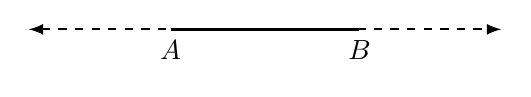
\begin{tikzpicture}[>=latex]
\draw[<->, dashed, thick](-3,0)--(3,0);
\draw[very thick](-1.2,0)node[below]{$A$}--(1.2,0)node[below]{$B$};
\end{tikzpicture}
	\caption{}
\end{figure}


如图1.6所示,由$A$点射向$B$点的光线可以由$A$向$B$的方
向无限延伸;而由$B$点射向$A$点的光线也可以由$B$向$A$的方向
无限延伸,所以对于空间任意两点$A$、$B$, 不但存在着唯一
的最短通路“直线段$AB$”,而且也唯一地确定了一条把直线
段$AB$两端无限延长的直线,这条直线就叫做由$A$、$B$两点所
确定的\textbf{直线},通常称为“直线$AB$”,而直线段$AB$是直线$AB$
介于A、B两点之间的那一段。

归纳上面的讨论,我们可以作出如下的总结:

\begin{enumerate}
	\item “位置”和“通路”是两个最原始的空间概念。
在几何学中,以点表示位置,以线表示通路。
\item 对于任何两点$A$、$B$, 在所有连结、$AB$的可能通路
中,存在唯一的最短通路,就是连结$A$、$B$两点的直线段。
\end{enumerate}

直线段$AB$也简称线段$AB$, 以后我们用符号$\overline{AB}$表示线段
$AB$。点$A$, 点$B$叫做线段$AB$的\textbf{端点}。有时,一条线段也可以
用一个小写字母来表示,例如线段$a$、线段$b$等(图1.7(1))。

\begin{figure}[htp]
	\centering
\begin{tikzpicture}
\begin{scope}
	\draw[|-|](0,0)node[left]{$A$}--(3,0)node[right]{$B$};
\draw[|-|](0,-1)--node[above]{$a$}(1.5,-1);
\draw[|-|](0,-2)--node[above]{$b$}(3,-2);
\node at (1.5,-2.5){(1)};
\end{scope}
\begin{scope}[xshift=6cm]
	\draw[|-|](0,0)node[left]{$A$}--(3,0)node[right]{$B$};
	\draw[|-|](0,-1.5)node[left]{$A'$}--(3,-1.5)node[right]{$B'$};
	\node at (0,-2){$(A)$}; \node at (3,-2){$(B)$};
	\node at (1.5,-2.5){(2)};
\end{scope}
\begin{scope}[yshift=-4cm]
	\draw[|-|](0,0)node[above]{$A$}--(3,0)node[above]{$B$};
	\node at (1.5,-2.5){(3)};
	\draw[|-|](0,-1.5)node[above]{$A'$}--(3,-1.5)node[above]{$B$};
	\draw[|-|](3,-1.5)--(4,-1.5)node[above]{$B'$};
	\node at (0,-2){$(A)$};
\end{scope}
\begin{scope}[xshift=6cm, yshift=-4cm]
	\draw[|-|](0,0)node[above]{$A$}--(3,0)node[above]{$B$};
	\node at (1.5,-2.5){(4)};
	\draw[|-|](0,-1.5)node[above]{$A'$}--(2,-1.5)node[above]{$B'$};
	\draw[|-|](2,-1.5)--(3,-1.5)node[above]{$B$};
	\node at (0,-2){$(A)$};
\end{scope}
\end{tikzpicture}
	\caption{}
\end{figure}

把$\overline{AB}$放在$\overline{A'B'}$上面,使点$A$和点$A'$重合,$\overline{AB}$沿着
$\overline{A'B'}$方向落下,那么有以下三种可能情况:
\begin{enumerate}
	\item 点$B$和点$B'$重合,这时$\overline{AB}=\overline{A'B'}$ (图1.7(2));
	\item 点$B$落在$A'$和$B'$之间,这时$\overline{AB}<\overline{A'B'}$ (图1.7(3));
	\item 点$B$落在$\overline{A'B'}$的延长线上,这时$\overline{AB}>\overline{A'B'}$ (图1.7(4)).
\end{enumerate} 


有一根拉直的绳子$\overline{AB}$, 如果把它分成长度相等的两段。
但是不许用尺来量,应怎么办?

同学们一定会想到,把绳子$\overline{AB}$
的两端点$A$、$B$重叠在一起,并且把绳子拉直,那么在绳子的中间就折出一
个$C$点来(图1.8(2)), 而被折成
的两段绳子$\overline{AC}$和$\overline{CB}$恰好长度相等,这就是说$C$点把$\overline{AB}$平分
了。所以我们把平分线段的点叫做\textbf{线段的中点}。如果点$C$是
$\overline{AB}$的中点,则$\overline{AB}=2\overline{AC}=2\overline{CB}$.

\begin{figure}[htp]\centering
    \begin{minipage}[t]{0.48\textwidth}
    \centering
\begin{tikzpicture}[>=latex, scale=1]
	\draw (0,0)node[above]{$A$}--(3,0)node[above]{$B$};
	\draw (0,-1)node[below]{$A$}--(1.5,-1)node[below]{$C$};
	\draw [dashed](1.5,-1)--(3,-1)node[below]{$B$};
	\node at (4,0){(1)};\node at (4,-1){(2)};
    \end{tikzpicture}
    \caption{}
    \end{minipage}
    \begin{minipage}[t]{0.48\textwidth}
    \centering
    \begin{tikzpicture}[>=latex, scale=1]
      \draw(0,0)node[left]{$A$}--(5,0)node[right]{$B$};
\tkzDefPoints{1/0/M, 2/0/C, 3.5/0/N}
\tkzDrawPoints(M,C,N)
\tkzLabelPoints[above](M,N)
\tkzLabelPoint[below](C){$C$}
\draw[|<->|, dashed](0,-1)--node[fill=white]{24厘米}(5,-1);


    \end{tikzpicture}
    \caption{}
    \end{minipage}
    \end{figure}



\begin{example}
	已知$\overline{AB}=24$厘米,点$C$在$\overline{AB}$上,点$M$、$N$分别是
	$\overline{AC}$和$\overline{CB}$的中点,求$\overline{MN}$的长度(见图1.9)。
\end{example}

\begin{solution}
\[\begin{split}
	\overline{MN}&=\overline{MC}+\overline{CN}=\frac{1}{2}\overline{AC}+\frac{1}{2}\overline{CB}\\
	&=\frac{1}{2}\left(\overline{AC}+\overline{CB}\right)=\frac{1}{2}\overline{AB}=12\text{厘米}
\end{split}\]
\end{solution}

\begin{enumerate}\setcounter{enumi}{2} 
	\item 线段可以向两端无限延长,这样就得到一条直线。一条直线可以用表示它上面任
	意两点的大写字母来表示,如直线$CD$. 有时为了简便,也可
	以在这条直线旁标以一个小写字母,如$\ell$,表示成
	直线$\ell $ (图1.10)。
	\item 对于任何两点$A$、$B$, 都存在着唯一一条通过$A$、$B$
	的直线。这个性质就简述为:\textbf{两点确定一条直线}。
\end{enumerate}

\begin{figure}[htp]
	\centering
\begin{tikzpicture}
\draw (0,0)--(5,0)node[right]{$\ell$};
\tkzDefPoints{1.5/0/C, 3.5/0/D}
\tkzDrawPoints(C,D)
\tkzLabelPoints[below](C,D)
\end{tikzpicture}
	\caption{}
\end{figure}

根据上述性质,我们可以说明其它有关的性质和问题。

\begin{example}
	如果两条直线$\ell$和$m$有一个公共点(交点)$A$(图1.11),它们还能有其它的公共点吗?为什么?
\end{example}

\begin{figure}[htp]
	\centering
	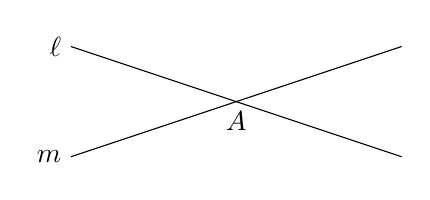
\begin{tikzpicture}[scale=.7]
		\draw (-3,1)node[left]{$\ell$}--(3,-1);
\draw(-3,-1)node[left]{$m$}--(3,1);
\node at (0,0)[below]{$A$};
	\end{tikzpicture}
	\caption{}
\end{figure}

\begin{solution}
除$A$点外,直线$\ell$和$m$不
能再有其它的公共点了。

因为,如
果还有另一个公共点$B$, 那么,$\ell$和$m$就都是通过$A$、$B$两点的直线。
但是通过$A$、$B$两点只有唯一的一条
直线,于是,$\ell$和$m$就是通过$A$、$B$两点的那条唯一的直线,
它们就不是两条不同的直线了。所以,它们除了$A$点外,不
可能再有其它的公共点了。

这件事实可以简述为:\textbf{两条相交直线确定一交点}。
\end{solution}


\begin{example}
	图1.12表示人和物之间放一隔板,使人不能直接
看到物的示意图,$A$表示物,$E$表示人眼,$\overline{BC}$表示隔板。为
了能看见物的形象,放置一面镜子,图中$g$表示镜面,这时
按图1.12(1)中隔板$\overline{BC}$的位置来说,人眼$E$便能看见物A的形象,这是为什么?但按图1.12(2)隔板$\overline{BC}$的位置
来说,人眼$E$便不能看到物$A$的形象,这又是为什么?
\end{example}

\begin{figure}[htp]
	\centering
\begin{tikzpicture}[>=latex]
\begin{scope}
\draw(0.5,0)node[left]{$g$}--(4.5,0);
\draw (1,1)node[above]{$A$}--(2,0)node[below]{$D$}--(4,2)node[right]{$E$};
\draw[dashed] (1,1)--(1,-1)node[below]{$A'$}--(2,0);
\node at (2.5,-2){(1)};
\draw[very thick](3,2.7)node[left]{$B$}--(3,1.2)node[left]{$C$};
\draw[->](1,1)--(1.5,.5); \draw[->](2,0)--(3.5,1.5);
\end{scope}

\begin{scope}[xshift=6cm]
	\draw(0.5,0)node[left]{$g$}--(4.5,0);
	\draw (1,1)node[above]{$A$}--(2,0)node[below]{$D$}--(4,2)node[right]{$E$};
	\draw[dashed] (1,1)--(1,-1)node[below]{$A'$}--(2,0);
	\node at (2.5,-2){(2)};
	\draw[very thick](3,2)node[left]{$B$}--(3,.5)node[right]{$C$};
	\draw[->](1,1)--(1.5,.5); \draw[->](2,0)--(2.5,.5);
	\end{scope}
\end{tikzpicture}
	\caption{}
\end{figure}

\begin{solution}
	按照镜面映象的道理,人眼$E$是从入射线$AD$和反射线$DE$看见$A$的形象的,而点$D$是点$E$和点$A$的象$A'$的连线
	$EA'$和$g$的交点,所以$A$的象$A'$是沿着直线$A'E$映入人眼
	$E$的。因为通过$A'$和$E$只有唯一的一条直线,于是$A'E$和隔板
	$\overline{BC}$不交(图1.12(1))时,在$E$处就看得见$A$的象$A'$, $A'E$和
	$\overline{BC}$相交,也就是被隔板$\overline{BC}$挡住(图1.12(2))时,在$E$处
	便看不见$A$的象$A'$了。
\end{solution}

\begin{example}
	如果在已知$\overline{AB}$上依次取99个点($C_1,C_2,C_3,\ldots,C_{99}$),那么$\overline{AB}$上一共有多少条以这些点为端点的线
	段?($\overline{AB}$也计算在内)
\end{example}	

\begin{solution}
	我们分以下几步来研究这个问题:

	第一,先进行观察、实验。因为每两个点就确定一条线段。因此,
\begin{enumerate}
	\item 在$\overline{AB}$上取一个点$C_1$时,我们看到图1.13(1)中共
	有3条线段$\overline{AB}$、$\overline{AC_1}$和$\overline{C_1B}$.

\begin{figure}[htp]
	\centering
\begin{tikzpicture}[yscale=1.3]
\foreach \x/\xtext in {0/(1),-1/(2),-2/(3),-3/(4),-4.5/(99)}
{
	\draw[|-|] (0,\x)node[below]{$A$}--(8,\x)node[below]{$B$};
	\node at (9,\x){$\xtext$};
}

\draw(2,0)node[below]{$C_1$}--(2,.1);
\draw(1.5,-1)node[below]{$C_1$}--(1.5,-1+.1);
\draw(3,-1)node[below]{$C_2$}--(3,-1+.1);

\foreach \x/\xtext in {1/C_1,2.5/C_2,4/C_3}
{
	\draw(\x,-2)node[below]{$\xtext$}--(\x,-2+.1);
}

\foreach \x/\xtext in {1/C_1,2.5/C_2,4/C_3, 5/C_4}
{
	\draw(\x,-3)node[below]{$\xtext$}--(\x,-3+.1);
}

\foreach \x/\xtext in {1.2/C_1,2/C_2,3.5/C_3,7/C_{99}}
{
	\draw(\x,-4.5)node[below]{$\xtext$}--(\x,-4.5+.1);
}
\node at (4,-3.8){$\vdots$};\node at (9,-3.8){$\vdots$};

\end{tikzpicture}
	\caption{}
\end{figure}

\item 在$\overline{AB}$上取两个点$C_1$、$C_2$时,我们看到图1.13(2)
中共有6条线段$\overline{AB}$、$\overline{AC_1}$、$\overline{C_1B}$、$\overline{AC_2}$、$\overline{C_2B}$和$\overline{C_1C_2}$.
\item 在$\overline{AB}$上取三个点$C_1$、$C_2$、$C_3$时,我们看到图1.13(3)中有10条线段(请同学们自己找出来)。
\end{enumerate}

第二,列表分析找规律
\begin{center}
	\begin{tabular}{cc}
\hline
$\overline{AB}$上取的点数 & $\overline{AB}$上线段的总数\\
\hline
1&3\\
2&6\\
3&10\\
$\vdots$&$\vdots$\\
99& ?\\
\hline
	\end{tabular}
\end{center}

从表上发现:
\begin{itemize}
\item 在$\overline{AB}$上取1个点时,$\overline{AB}$上的线段总数$3=1+2$,
\item 在$\overline{AB}$上取2个点时,$\overline{AB}$上的线段总数$6=1+2+3$,
\item 在$\overline{AB}$上取3个点时,$\overline{AB}$上的线段总数$10=1+2+3+4$。
\end{itemize}

这时,如果在$\overline{AB}$上取4个点,那么$\overline{AB}$上共有多少条线段
呢?由上面发现的规律,可以猜想是$1+2+3+4+5=15$, 数
一下图1.13(4)中的线段数,恰好是15条。这样自然要
问:当在$\overline{AB}$上取99个点时,将会有怎样的结果呢?

第三,归纳、计算

如果在$\overline{AB}$上取99个点,设这时$\overline{AB}$上的线段总数为$S$,
由在第二中发现的规律,不难得出:
\[S=1+2+3+4\cdots +(99+1)=1+2+3+4\cdots +100\]

这是一个很有趣的计算题,如果按顺序加起来,计算是
很麻烦的,我们动动脑筋能否有简便的计算方法呢?

由于$S=1+2+3+\cdots +98+99+100$,也就是:
\[S=100+99+98+\cdots +3+2+1\]
$\therefore\quad 2S=\underbrace{101+101+101\cdots+101+101+101}_{100\text{项}}=100\x 101$

$\therefore\quad S=\frac{100\x 101}{2}=5050$
\end{solution}

\begin{figure}[htp]
	\centering
	\begin{tikzpicture}[scale=.7]
\tkzDefPoints{0/0/B, 6/0/C, 5/3/D, 2/3/A}
\tkzDrawPolygon(A,B,C,D)
\tkzLabelPoints[left](A,B)
\tkzLabelPoints[right](C,D)
\draw(B)--(D);\node at (3.2,1.8)[below]{$O$};
\draw(A)--(C);		
	\end{tikzpicture}
	\caption*{第1题}
\end{figure}

\begin{ex}
\begin{enumerate}
	\item 图中有几条线段,把它们都写出来。
	\item $A$、$B$、$C$三点不在一条直线上,通过其中任何两点画一
	条直线,一共能画出几条直线?
	\item $A$、$B$、$C$、$D$四点中,任何三点都不在一条直线上,通过
	其中任何两点画一条直线,一共能画出几条直线?
	\item 如果$A$、$B$、$C$、$D$、$E$五点中任何三点都不在一条直线
上,通过其中任何两点画一条直线,那么一共能画多少条直线?
	\item 如果有100个点,其中任何三点都不在一条直线上,通
	过其中任何两点画一条直线,那么一共能画多少条直线?
	\item 工人师付在用方砖铺地时,常常打两个木桩,拉线来铺
	砖,这样砖就铺得整齐,这是根据了什么道理?
\item 如果有两个小孩甲、乙在对话,甲问乙:“你的家住在哪
里?”乙回答说:“我的家住在直线$AB$的尽头。”试问
你能沿着直线$AB$找到乙的家吗?为什么?
\item 参看例1.4的归纳、计算,如果在$\overline{AB}$上取$n$个点。那么
$\overline{AB}$上一共有多少条线段?($\overline{AB}$也计算在内)
\item 已知:$\overline{MN}=100$米,$P$点在$\overline{MN}$上,$\overline{MP=45}$米,$S$点是
$\overline{PN}$的中点,求$\overline{PS}$的长度是多少米?
\item 在例1.1中,$\overline{MN}$的长度与$C$点在$\overline{AB}$上的位置有无
关系?
\end{enumerate}
\end{ex}


\subsection{长度的度量}
在给定两点$A$、$B$之间的所有通路之中,以$AB$为最短,
它的“长度”就叫做$A$、$B$\textbf{两点间的距离}。所以,两点间的
距离是连结这两点的线段的长。

长度是我们经常用的一种几何量,现在让我们分别从实
用和数学的观点稍微细致地分析一下“长度”这种几何量的
直观含义,并且谈一谈长度的度量。

一般来说,常用的量基本上可以归成两类:其中一类,例
如一群羊、一堆蛋,它们具有天然的个别单元,即一只羊、一
个蛋。处理这种量,我们只要去数一数它们的“个数”就可以
了。因为它们是可数的。用来数“个数”的数学体系就是我
们在代数学中一开始就详加讨论的自然数系:$\{1,2,3,\ldots\}$. 另一类,例如我们现在要讨论的长度等,这种量虽然不具有
天然个别单元,但是,具有一个基本特点:可以无限细分。
例如,任给一个线段,不管它怎样短,还是可以把它分割成
更短的线段。因此,这种量不可能有天然不可分割的单元,
我们处理这种量的办法就是度量。

因为长度这种量并不具有天然不可分割的单位,所以,
我们只好选用人为的长度单位。例如“米”就是世界上通用
的长度单位。取定长度单位以后,要度量一条线段的长度,
也就是要求得它和长度单位之间的“比值”。例如取定长
度单位为米,所求得的比值是1237:1000,就说这条线段的长
度是1.237米。但是在实践中,这个比值是怎样求出来的
呢?先举几个简单的实例看一看。

\begin{example}
设长度单位是$u$, 所要度量的线段是$a$ (图1.14).
线段$a$恰好可以分割成5段和$u$等长的线段,那么所求的比
值是5, $a$的长度就是$5u$. 

一般地说,如果所要度量的线段$a$恰好可以分割成$m$段
和$u$等长的线段,那末所求的比值就是整数$m$, $a$的长度就是$mu$.
\end{example}

\begin{figure}[htp]\centering
    \begin{minipage}[t]{0.48\textwidth}
    \centering
\begin{tikzpicture}[>=latex, scale=1]
       \draw [|-|](0,0)--(1,0);
	   \draw [|-|](0,-1)--(5,-1);
	   \node at (-.5,0){$u:$};
	   \node at (-.5,-1){$a:$};
	   \foreach \x in {1,2,3,4}
	   {
\draw (\x,-1)--(\x,-.9);
	   }
    \end{tikzpicture}
    \caption{}
    \end{minipage}
    \begin{minipage}[t]{0.48\textwidth}
    \centering
    \begin{tikzpicture}[>=latex, scale=1]
		\draw [|-|](0,0)--(3,0);
		\draw [|-|](0,-1)--(1,-1);
		\node at (-.5,0){$u:$};
		\node at (-.5,-1){$b:$};
		\foreach \x in {1,2}
		{
 \draw (\x,.1)--(\x,0);
		}
    \end{tikzpicture}
    \caption{}
    \end{minipage}
    \end{figure}

\begin{example}
设长度单位是$u$, 所要度量的线段是$b$ (图1.15) 单
位长$u$恰好可以分割成3段和$b$等长的线段,那么所求的比
值是$\frac{1}{3}$, $b$的长度就是$\frac{1}{3}u$. 

一般地说,如果长度单位$u$恰
好可以分割成$n$段和$b$等长的线
段,那么所求的比值是$\frac{1}{n}$
,$b$的长度就是$\frac{1}{n}u$
\end{example}

\begin{example}
	设长度单位是$u$, 所要度量的线段是$c$ (图1.16). $c$比$4u$长些,但又比$5u$短些,如果我们把$u$三等分,
	线段$c$截取4段$u$后所余的一段恰好是$\frac{1}{3}u$的2倍,那么c的
	长度就是$4\frac{2}{3}u$.

\begin{figure}[htp]
	\centering
\begin{tikzpicture}
\draw[|-|] (0,0)node[left]{$b:$}--(4.667,0);
\draw[|-|] (0,1)node[left]{$v:$}--(1,1);
\end{tikzpicture}
	\caption{}
\end{figure}

一般地说,如果把长度单位$u$适当地等分成$n$段,即每
一段$u'$的长度是$\frac{1}{n}\cdot u$, 所要量的线段$c$恰好可以分割成
$m$段和线段$u'$等长的线段,那么$c$的长度就是$\frac{m}{n}u$。

在例1.7中,用长度单位$u$去度量$c$时,怎样才能知道在$c$
上截取4段$u$后,所余的一段恰好是$u$的$\frac{1}{3}$的整数倍?实际上
可以这样来确定:在$c$上截取4段$u$后,以所余的一段$\overline{C_4D}$去
量$u$, 在$u$上截去一段$\overline{C_4D}$后,所余的一段$\overline{U_1V}$又较$\overline{C_4D}$短,
这时再以$\overline{U_1V}$去度量$\overline{C_4D}$, 恰好$\overline{C_4D}$是$\overline{U_1V}$的2倍。这样便
看出$\overline{U_1V}$是$u$的$\frac{1}{3}$,把$u$三等分后,$\overline{C_4D}$就恰好是$\frac{1}{3}u$的2
倍了。
\end{example}

\begin{example}
	设长度单位是$u$, 求线段$d$的长度(图1.17)。
\begin{figure}[htp]
	\centering
\begin{tikzpicture}[xscale=4]
	\draw[|-|] (0,1)node[left]{$u:$}--(1,1)node[below]{$V$};
	\draw[|-|] (0,0)node[left]{$d:$}--(2.42,0)node[right]{$E$};
	\draw(1,0)--(1,.1); \draw(2,0)node[below]{$D_2$}--(2,.1);
	\draw(2.333,0)node[below]{$F_2$}--(2.333,.1);
	\draw(.42,1)--(.42,1.1);  \draw(.84,1.1)--(.84,1)node[below]{$U_2$};
	\draw(2.16,0)--(2.16,0.1);
	\draw(.84+.08,1.1)--(.84+.08,1);
\end{tikzpicture}	
	\caption{}
\end{figure}
\end{example}

\begin{solution}
	在$d$上用圆规截取2段$u$后,所余的一段$\overline{D_2E}$较$u$
短;在$u$上截取2段$\overline{D_2E}$后,所余的$\overline{U_2V}$较$\overline{D_2E}$短;在$\overline{D_2E}$
上截取2段$\overline{U_2V}$后,所余的一段$\overline{F_2E}$较$\overline{U_2V}$短;但$\overline{U_2V}$恰
好是$\overline{F_2E}$的2倍。于是
\[\begin{split}
	\overline{D_2E}&=\overline{D_2F_2}+\overline{F_2E}=2\overline{U_2V}+\overline{F_2E}\\
&=2\cdot 2\overline{F_2E}+\overline{F_2E}=5\overline{F_2E}
\end{split}\]
\[u=2\overline{D_2E}+\overline{U_2V}=2-5\overline{F_2E}+2\overline{F_2E}=12\overline{F_2E}\]
$\therefore\quad \overline{F_2E}=\frac{1}{12}u,\quad \overline{D_2E}=\frac{5}{12}u,\quad d=2\frac{5}{12}u$
\end{solution}


由例1.7和例1.8可以看出,当被度量线段($c$和$d$)不能恰好
被分割而成为长度单位的整数倍,也就是它们不能被长度单
位量尽时,都是求出另一条线段(例1.7中是$\overline{U_1V}$, 例1.8中是$\overline{F_2E}$),使得它能量尽长度单位和被量线段。再按例1.6的方
法求出以长度单位为单位的这条线段的长度,然后便可求出
原来被量线段的长度了。

能够量尽两条线段$a$和$b$的线段,我们叫它做线段$a$和$b$的
\textbf{公度}。两条线段的公度中最长的,叫做\textbf{这两条线段的最大公
度}。$\overline{U_1V}$和$\overline{F_2E}$就分别是线段$u$和$c$, $u$和$d$的最大公度。在
例1.5中线段$u$就是线段$u$和$a$的最大公度;例1.6中的线段$b$就是线
段$u$和$b$的最大公度,象例1.7、例1.8中求线段$u$和$c$、$u$和$d$的最
大公度的方法,叫做\textbf{辗转相截法}。

通过上面各例,我们很自然地会想到:任何两条线段
$a, b$, 它们的长度比值是否总是一个分数(整数也可看作
分数)?换句话说,对于任何两条线段$a$、$b$, 是否存在着它
们的公度?

这个问题从正、反两面来分析它的重要性。首先,如果
任何两条线段的长度的比值总是一个分数,那么分数全体
(即代数开始所讲的有理数)就足以处理长度的度量问题
了。其次,反过来说,如果两条线段的长度的比值不一定是
分数,那么有理数就不足以处理长度的度量问题。因而我们
就得学会一种含有“非分数”的数系才能充分解决度量问
题。这个问题是整个数学发展史上的一件大事,我们以后再
详细讨论。

\begin{ex}
\begin{enumerate}
	\item 已知线段$a$、$b$、$u$, 其中线段$a=9u$, $b=3u$, 问线段$a$、$b$的最大公度是线段$u$的几倍?
	\item 已知线段$a=48$毫米,$b=18$毫米。先用辗转相截法求出
	$a$、$b$的最大公度,并量它等于多少毫米;再用求最大公
	约数的辗转相除法求出48、18的最大公约数。比较前后所得
	的结果。
	\item 根据图形填写下面空白:
\begin{enumerate}
	\item $\overline{AC}=\overline{BC}+(\qquad)$	
	\item	$\overline{CD}=\overline{AD}-(\qquad)$	
	\item $\overline{AC}+\overline{CD}=(\qquad)+\overline{BD}$
\end{enumerate}
\begin{center}
	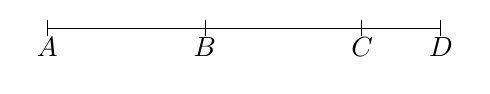
\begin{tikzpicture}
	\draw[|-|](0,0)node[below]{$A$}--(5,0)node[below]{$D$};
	\draw[|-|](2,0)node[below]{$B$}--(4,0)node[below]{$C$};	
	\end{tikzpicture}
\end{center}
\end{enumerate}
\end{ex}

\subsection{直线和平面}
在空间,另一种常见的形象就是各种各样的面。例如地
球的表面,它的整体看起来是一个略为扁平的球面,而局部
的形象又随着当地的地貌而不同。有的地方是一片原,有
的地方是起伏的丘陵,有的地方是一片湖面,也有的地方是
崇山峻岭和深谷。又如教室的一面墙壁,上课用的黑板,以
及桌面等,看起来又都是“平直”的面。

通常检查一个桌面是否“平直”,最简单的方法就是用一
根直尺放在桌面上(图1.18),如果放在任何位置上,直
尺的边都和桌面密合,那么桌面就是“平直”的。我们就说
桌面是平面。但是象图1.19的面上,虽然直尺放在$\ell_1,\ell_2,\ldots,\ell_n$等位置时,直尺边和这个面密合,而在$AB$位置上直尺
边和面就不密合了。这就是说并不是在任何位置上直尺的边
总和这个面密合,这个面不是一个平面,实际上是一个曲
面。

在几何学的讨论中,平面就是一个到处平直而且向各个
方向无限延展的面,它的特点就是在它上面任取两点$A$和$B$
(图1.20),直线$AB$就完全在这个平面内。


我们观察一扇门,把它看作平面的一部分,那么它的轴
线既在墙壁的平面内(图1.21),又在这扇门所在的平面
内,不可能连结两个“合页”的直线不都在这两个平面内。推动这扇门,它每到一个新的位置都表现了通过轴线的一个平面。这些事实说明了:
\textbf{空间相交的两个平面的“交界”是一条直
线。通过一条直线可有无数个平面。}

\begin{ex}
\begin{enumerate}
	\item 举出一条直线和一个平面没有公共点的实例,以及一条直
	线和一个平面只有一个公共点的实例。
	\item 一点在一平面内,而其它的点都不在这个平面内,这种实例有\item 举出两个平面没有公共点的实例。
	\item 两个平面只有一个公共点的实例存在吗?
	\item 如果空间被平面$\alpha$分成的两部分之一中,有一只小虫子$A$,这只小虫子$A$要爬到	被平面所分空间的另一部分去,假如它
	不穿过平面$\alpha$,能过去吗?为什么?
\begin{center}
	\begin{tikzpicture}
		
	\end{tikzpicture}
\end{center}
\end{enumerate}
\end{ex}

同学们作这样一个实验,张开手指,使拇指、食指和中指的尖
这三点不在一条直线上,拿一张硬纸(它代表一个平
面)往三个指尖上放,看看它是否能同时通过三个指尖?再
拿一张硬纸仍然这样放,看这两张硬纸是否重合?这种特点
对于一个指尖,两个指尖也适合吗?再使母指、食指、中
指,无名指的指尖这四点不在一条直线上,看看能否保证总
有一张硬纸同时通过这四点?仿照“两点确定一条直线”的
特点,同学们能否总结出几个点确定一个平面的结论?

通过上面的实验,我们得出平面的另一个基本性质:
\textbf{空间不共线三点确定一个平面。}

同学们还可进一步思考以下的问题:
\begin{enumerate}
	\item 一直线及直线外一点能确定一个平面吗?
	\item 相交的两条直线能确定一个平面吗?
\end{enumerate}

\section*{习题1.1}
\addcontentsline{toc}{subsection}{习题1.1}
\begin{enumerate}
	\item 什么是线段?什么是直线?两者有什么区别?
	\item 什么是线段的中点?如果有一根笔直的铁棍,
	假如用$\overline{AB}$
	来表示它,不用尺量,也不许把它折弯,你有没有办法找
	出$\overline{AB}$所表示的这根铁棍的中点来?
	\item 请同学们复习一下小学学过的公制、市制两种长度单位,
	并填下表:










\end{enumerate}



